\documentclass{article}
\usepackage{geometry}
 \geometry{
 a4paper,
 total={170mm,257mm},
 left=20mm,
 top=20mm,
 }

 \usepackage{caption}
\usepackage[export]{adjustbox} %% for picture frame
\usepackage[english]{babel}
\usepackage[utf8]{inputenc}
\usepackage{fancyhdr}

%%%question enviroment 

%%% Question Environment%%%  use 
%%% Question Environment%%%  use 
%%% Question Environment%%%  use \input{./QueENV.tex}   to include
%% Use \begin{Q}....\end{Q}

\newcounter{QC}
\setcounter{QC}{1}
\newenvironment{Q}[1]{
    \section{Question -\arabic{QC}} \stepcounter{QC}{\large\textbf{#1}}
}

%%% Question Environment%%%

   to include
%% Use \begin{Q}....\end{Q}

\newcounter{QC}
\setcounter{QC}{1}
\newenvironment{Q}[1]{
    \section{Question -\arabic{QC}} \stepcounter{QC}{\large\textbf{#1}}
}

%%% Question Environment%%%

   to include
%% Use \begin{Q}....\end{Q}

\newcounter{QC}
\setcounter{QC}{1}
\newenvironment{Q}[1]{
    \section{Question -\arabic{QC}} \stepcounter{QC}{\large\textbf{#1}}
}

%%% Question Environment%%%



\pagestyle{fancy}
\fancyhf{}
\rhead{\textit{LAB-3}}
\lhead{\textit{Pul074BEX004}}
\rfoot{\thepage}

%%% format and command for lab ans c and assembly

%%% Formating And Command for Embedded Lab   Assambly & C%%%


%%% Formatting And Command for Embedded Lab   Assembly & C%%%
%% 
%%% Formating And Command for Embedded Lab   Assambly & C%%%


%%% Formatting And Command for Embedded Lab   Assembly & C%%%
%% 
%%% Formating And Command for Embedded Lab   Assambly & C%%%


%%% Formatting And Command for Embedded Lab   Assembly & C%%%
%% \input{./asm c.tex}

%% \anscode{problem no. like 1,2,3...}{assembly code file }{ code file}


\usepackage{listings}
\usepackage{multicol}
\usepackage{mdframed}

\renewcommand{\lstlistlistingname}{List of Codes}
\renewcommand{\lstlistingname}{Code}


\setlength{\columnsep}{0.5cm}

\usepackage{xcolor}
\definecolor{codegreen}{rgb}{0,0.6,0}
\definecolor{codegray}{rgb}{0.4,0.4,0.4}
\definecolor{codepurple}{rgb}{0.58,0,0.82}
%\definecolor{backcolour}{rgb}{0.95,0.99,0.92}
\definecolor{backcolour}{rgb}{0,0,0}


\lstdefinestyle{customa}{
  backgroundcolor=\color{backcolour},   commentstyle=\color{codegreen},
  keywordstyle=\color{magenta},
  numberstyle=\tiny\color{codegray},
  stringstyle=\color{codepurple},
  basicstyle=\ttfamily\small\color{white},
  breakatwhitespace=false,
  breaklines=true,
  captionpos=b,
  morekeywords={MOV,ADD,ADDC,ACALL,INC,DJNZ,AJMP,RET,END,ORG,RR,JNC,SUBB,JC,DEC,ANL,SWAP,MUL,DIV,CLR,SETB},
  keepspaces=true,
  numbers=left,
  numbersep=5pt,
  showspaces=false,
  showstringspaces=false,
  showtabs=false,
  tabsize=4
}

\lstdefinestyle{customc}{
  backgroundcolor=\color{backcolour},   commentstyle=\color{codegreen},
  keywordstyle=\color{cyan},
  numberstyle=\tiny\color{codegray},
  stringstyle=\color{codepurple},
  basicstyle=\ttfamily\footnotesize\color{white},
  breakatwhitespace=false,
  breaklines=true,
  captionpos=b,
  keepspaces=true,
  language=C,
  numbers=left,
  numbersep=5pt,
  showspaces=false,
  showstringspaces=false,
  showtabs=false,
  tabsize=3
}




\newcommand {\anscode}[3]{

  \begin{center}
    \textbf{Assembly}
  \end{center}

  \begin{multicols}{2}
    \lstinputlisting[style=customa,nolol]{#2}
  \end{multicols}

  \begingroup
  \captionof{lstlisting}{Problem no. #1 Assembly}
  \endgroup


  \vspace{2 em}


  \begin{center}
    \textbf{C language }
  \end{center}
  \begin{multicols}{2}
    \lstinputlisting[style=customc,nolol]{#3}
  \end{multicols}

  \begingroup
  \captionof{lstlisting}{Problem no. #1 C language}
  \endgroup
}

%%% Formating And Command for Embedded Lab  Assambly & C%%%

%% \anscode{problem no. like 1,2,3...}{assembly code file }{ code file}


\usepackage{listings}
\usepackage{multicol}
\usepackage{mdframed}

\renewcommand{\lstlistlistingname}{List of Codes}
\renewcommand{\lstlistingname}{Code}


\setlength{\columnsep}{0.5cm}

\usepackage{xcolor}
\definecolor{codegreen}{rgb}{0,0.6,0}
\definecolor{codegray}{rgb}{0.4,0.4,0.4}
\definecolor{codepurple}{rgb}{0.58,0,0.82}
%\definecolor{backcolour}{rgb}{0.95,0.99,0.92}
\definecolor{backcolour}{rgb}{0,0,0}


\lstdefinestyle{customa}{
  backgroundcolor=\color{backcolour},   commentstyle=\color{codegreen},
  keywordstyle=\color{magenta},
  numberstyle=\tiny\color{codegray},
  stringstyle=\color{codepurple},
  basicstyle=\ttfamily\small\color{white},
  breakatwhitespace=false,
  breaklines=true,
  captionpos=b,
  morekeywords={MOV,ADD,ADDC,ACALL,INC,DJNZ,AJMP,RET,END,ORG,RR,JNC,SUBB,JC,DEC,ANL,SWAP,MUL,DIV,CLR,SETB},
  keepspaces=true,
  numbers=left,
  numbersep=5pt,
  showspaces=false,
  showstringspaces=false,
  showtabs=false,
  tabsize=4
}

\lstdefinestyle{customc}{
  backgroundcolor=\color{backcolour},   commentstyle=\color{codegreen},
  keywordstyle=\color{cyan},
  numberstyle=\tiny\color{codegray},
  stringstyle=\color{codepurple},
  basicstyle=\ttfamily\footnotesize\color{white},
  breakatwhitespace=false,
  breaklines=true,
  captionpos=b,
  keepspaces=true,
  language=C,
  numbers=left,
  numbersep=5pt,
  showspaces=false,
  showstringspaces=false,
  showtabs=false,
  tabsize=3
}




\newcommand {\anscode}[3]{

  \begin{center}
    \textbf{Assembly}
  \end{center}

  \begin{multicols}{2}
    \lstinputlisting[style=customa,nolol]{#2}
  \end{multicols}

  \begingroup
  \captionof{lstlisting}{Problem no. #1 Assembly}
  \endgroup


  \vspace{2 em}


  \begin{center}
    \textbf{C language }
  \end{center}
  \begin{multicols}{2}
    \lstinputlisting[style=customc,nolol]{#3}
  \end{multicols}

  \begingroup
  \captionof{lstlisting}{Problem no. #1 C language}
  \endgroup
}

%%% Formating And Command for Embedded Lab  Assambly & C%%%

%% \anscode{problem no. like 1,2,3...}{assembly code file }{ code file}


\usepackage{listings}
\usepackage{multicol}
\usepackage{mdframed}

\renewcommand{\lstlistlistingname}{List of Codes}
\renewcommand{\lstlistingname}{Code}


\setlength{\columnsep}{0.5cm}

\usepackage{xcolor}
\definecolor{codegreen}{rgb}{0,0.6,0}
\definecolor{codegray}{rgb}{0.4,0.4,0.4}
\definecolor{codepurple}{rgb}{0.58,0,0.82}
%\definecolor{backcolour}{rgb}{0.95,0.99,0.92}
\definecolor{backcolour}{rgb}{0,0,0}


\lstdefinestyle{customa}{
  backgroundcolor=\color{backcolour},   commentstyle=\color{codegreen},
  keywordstyle=\color{magenta},
  numberstyle=\tiny\color{codegray},
  stringstyle=\color{codepurple},
  basicstyle=\ttfamily\small\color{white},
  breakatwhitespace=false,
  breaklines=true,
  captionpos=b,
  morekeywords={MOV,ADD,ADDC,ACALL,INC,DJNZ,AJMP,RET,END,ORG,RR,JNC,SUBB,JC,DEC,ANL,SWAP,MUL,DIV,CLR,SETB},
  keepspaces=true,
  numbers=left,
  numbersep=5pt,
  showspaces=false,
  showstringspaces=false,
  showtabs=false,
  tabsize=4
}

\lstdefinestyle{customc}{
  backgroundcolor=\color{backcolour},   commentstyle=\color{codegreen},
  keywordstyle=\color{cyan},
  numberstyle=\tiny\color{codegray},
  stringstyle=\color{codepurple},
  basicstyle=\ttfamily\footnotesize\color{white},
  breakatwhitespace=false,
  breaklines=true,
  captionpos=b,
  keepspaces=true,
  language=C,
  numbers=left,
  numbersep=5pt,
  showspaces=false,
  showstringspaces=false,
  showtabs=false,
  tabsize=3
}




\newcommand {\anscode}[3]{

  \begin{center}
    \textbf{Assembly}
  \end{center}

  \begin{multicols}{2}
    \lstinputlisting[style=customa,nolol]{#2}
  \end{multicols}

  \begingroup
  \captionof{lstlisting}{Problem no. #1 Assembly}
  \endgroup


  \vspace{2 em}


  \begin{center}
    \textbf{C language }
  \end{center}
  \begin{multicols}{2}
    \lstinputlisting[style=customc,nolol]{#3}
  \end{multicols}

  \begingroup
  \captionof{lstlisting}{Problem no. #1 C language}
  \endgroup
}

%%% Formating And Command for Embedded Lab  Assambly & C%%%
%%%%>>>>>>>........
%%%%%% include  Titles.%%%% use \input{./CP}%%%
%%%use """"""""    \CP{}{}{}{}   """" %%%% and 4 argument to craete Title page 
%%%%%%%%%%%%%%%%%%%%%%%%%%%%%%%%%%%%%%%%%%%%%%%%%%%%%%%%%%%%%%%%%
%%%argument number
%% 1=major header ## Course name 
%% 2=minor4 heading ## lab/assignmet no
%% 3=Title  ## Assignment or Lab title
%% 4=submitted to::## input receiver Name"
%%%%%%%%%%%%%%%%%%%%%%%%%%%%%%%%%%%%%%%%%%%%%%%%%%%%%%%%%%%%%%%%%


\usepackage{mathpazo} % Palatino font
\usepackage{graphicx}
\usepackage{float}

%%% format and command for lab ans c and assembly

\newcommand{\HRule}{\rule{\linewidth}{0.4mm}} % Defines a new command for horizontal lines, change thickness here



%----------------------------------------------------------------------------------------
%	TITLE PAGE
%----------------------------------------------------------------------------------------


\newcommand{\CP}[4]{ \begin{titlepage} % Suppresses displaying the page number on the title page and the subsequent page counts as page 1
		%%%%  univerdity logo%%
		\begin{figure}[H]
			\centering
			
\includegraphics[scale=0.13]{tulogo.jpg}
		\end{figure}
		%%% end university logo

		\center % Centre everything on the page

		%------------------------------------------------
		%	Headings
		%------------------------------------------------

		\textsc{\huge Institute of Engineering \\ Central Campus,Pulchowk}\\[1.5cm] % Main heading such as the name of your university/college

		\textsc{\Large #1}\\[0.5cm] % Major heading such as course name

		\textsc{\large #2}\\[0.5cm] % Minor heading such as assignment no./ lab no.

		%------------------------------------------------
		%	Title
		%------------------------------------------------

		\HRule\\[0.4cm]

		{\Huge\bfseries #3}\\[0.4cm] % Title of your document

		\HRule\\[1.5cm]

		%------------------------------------------------
		%	Author(s)
		%------------------------------------------------
		\vfill\vfill
		\begin{minipage}{0.4\textwidth}
			\begin{flushleft}
				\large{
				\textbf{Submitted BY:}\\
				{\normalsize AMRIT PRASAD PHUYAL}\\ % NAME
				{\normalsize Roll: PULL074BEX004}} % Roll
			\end{flushleft}
		\end{minipage}
		~
		\begin{minipage}{0.4\textwidth}
			\begin{flushright}
				\large
				\textbf{Submitted To:}\\
				{ \normalsize{#4}\\ }% recepent's  Name 
				{\normalsize Department of Electronics and Computer Engineering}
			\end{flushright}
		\end{minipage}

		%------------------------------------------------
		%	Date
		%------------------------------------------------

		\vfill\vfill\vfill % Position the date 3/4 down the remaining page

		{\large\today} % Date, change the \today to a set date if you want to be precise

		\vfill % Push the date up 1/4 of the remaining page

	\end{titlepage}
}

\begin{document}

%----------------------------------------------------------------------------------------
%	TITLE PAGE
%----------------------------------------------------------------------------------------
\CP{Embedded system}{LAB \#3}
{Programming Timers of 8051/8052 Microcontroller}
{Department of Electronics and Computer Engineering}




%----------------------------------------------------------------------------------------
\pagenumbering{gobble}
\tableofcontents
\pagebreak
\listoffigures
\pagebreak
\lstlistoflistings
\pagebreak
\pagenumbering{arabic}
\section{Introduction}
\subsection{Microcontroller}

A microcontroller is an integrated circuit ( IC), usually via an MPU, memory and certain peripherals, to control other parts of an electronic system .
These devices are optimized for embed-in applications that require agile and agile processing, digital, analog or electromechanical interactions.
\subsection{8051 Microcontroller}
In 1981, Intel introduced an 8-bit microcontroller called the 8051. It was referred as system on a chip because it had 128 bytes of RAM, 4K byte of on-chip ROM,
two timers, one serial port, and 4 ports (8-bit wide), all on a single chip.\\\\
The different features of the 8051 microcontroller include:
\begin{itemize}
    \item 4KB bytes on-chip program memory (ROM)
    \item 128 bytes on-chip data memory (RAM)
    \item Four register banks
    \item 128 user defined software flags
    \item 8-bit bidirectional data bus
    \item 16-bit unidirectional address bus
    \item 32 general purpose registers each of 8-bit
    \item 16 bit Timers (usually 2, but may have more or less)
    \item Three internal and two external Interrupts
    \item Four 8-bit ports,(short model have two 8-bit ports)
    \item 16-bit program counter and data pointer
    \item 8051 may also have a number of special features such as UARTs, ADC, Op-amp, etc.
\end{itemize}
\begin{figure}[H]
    \centering
    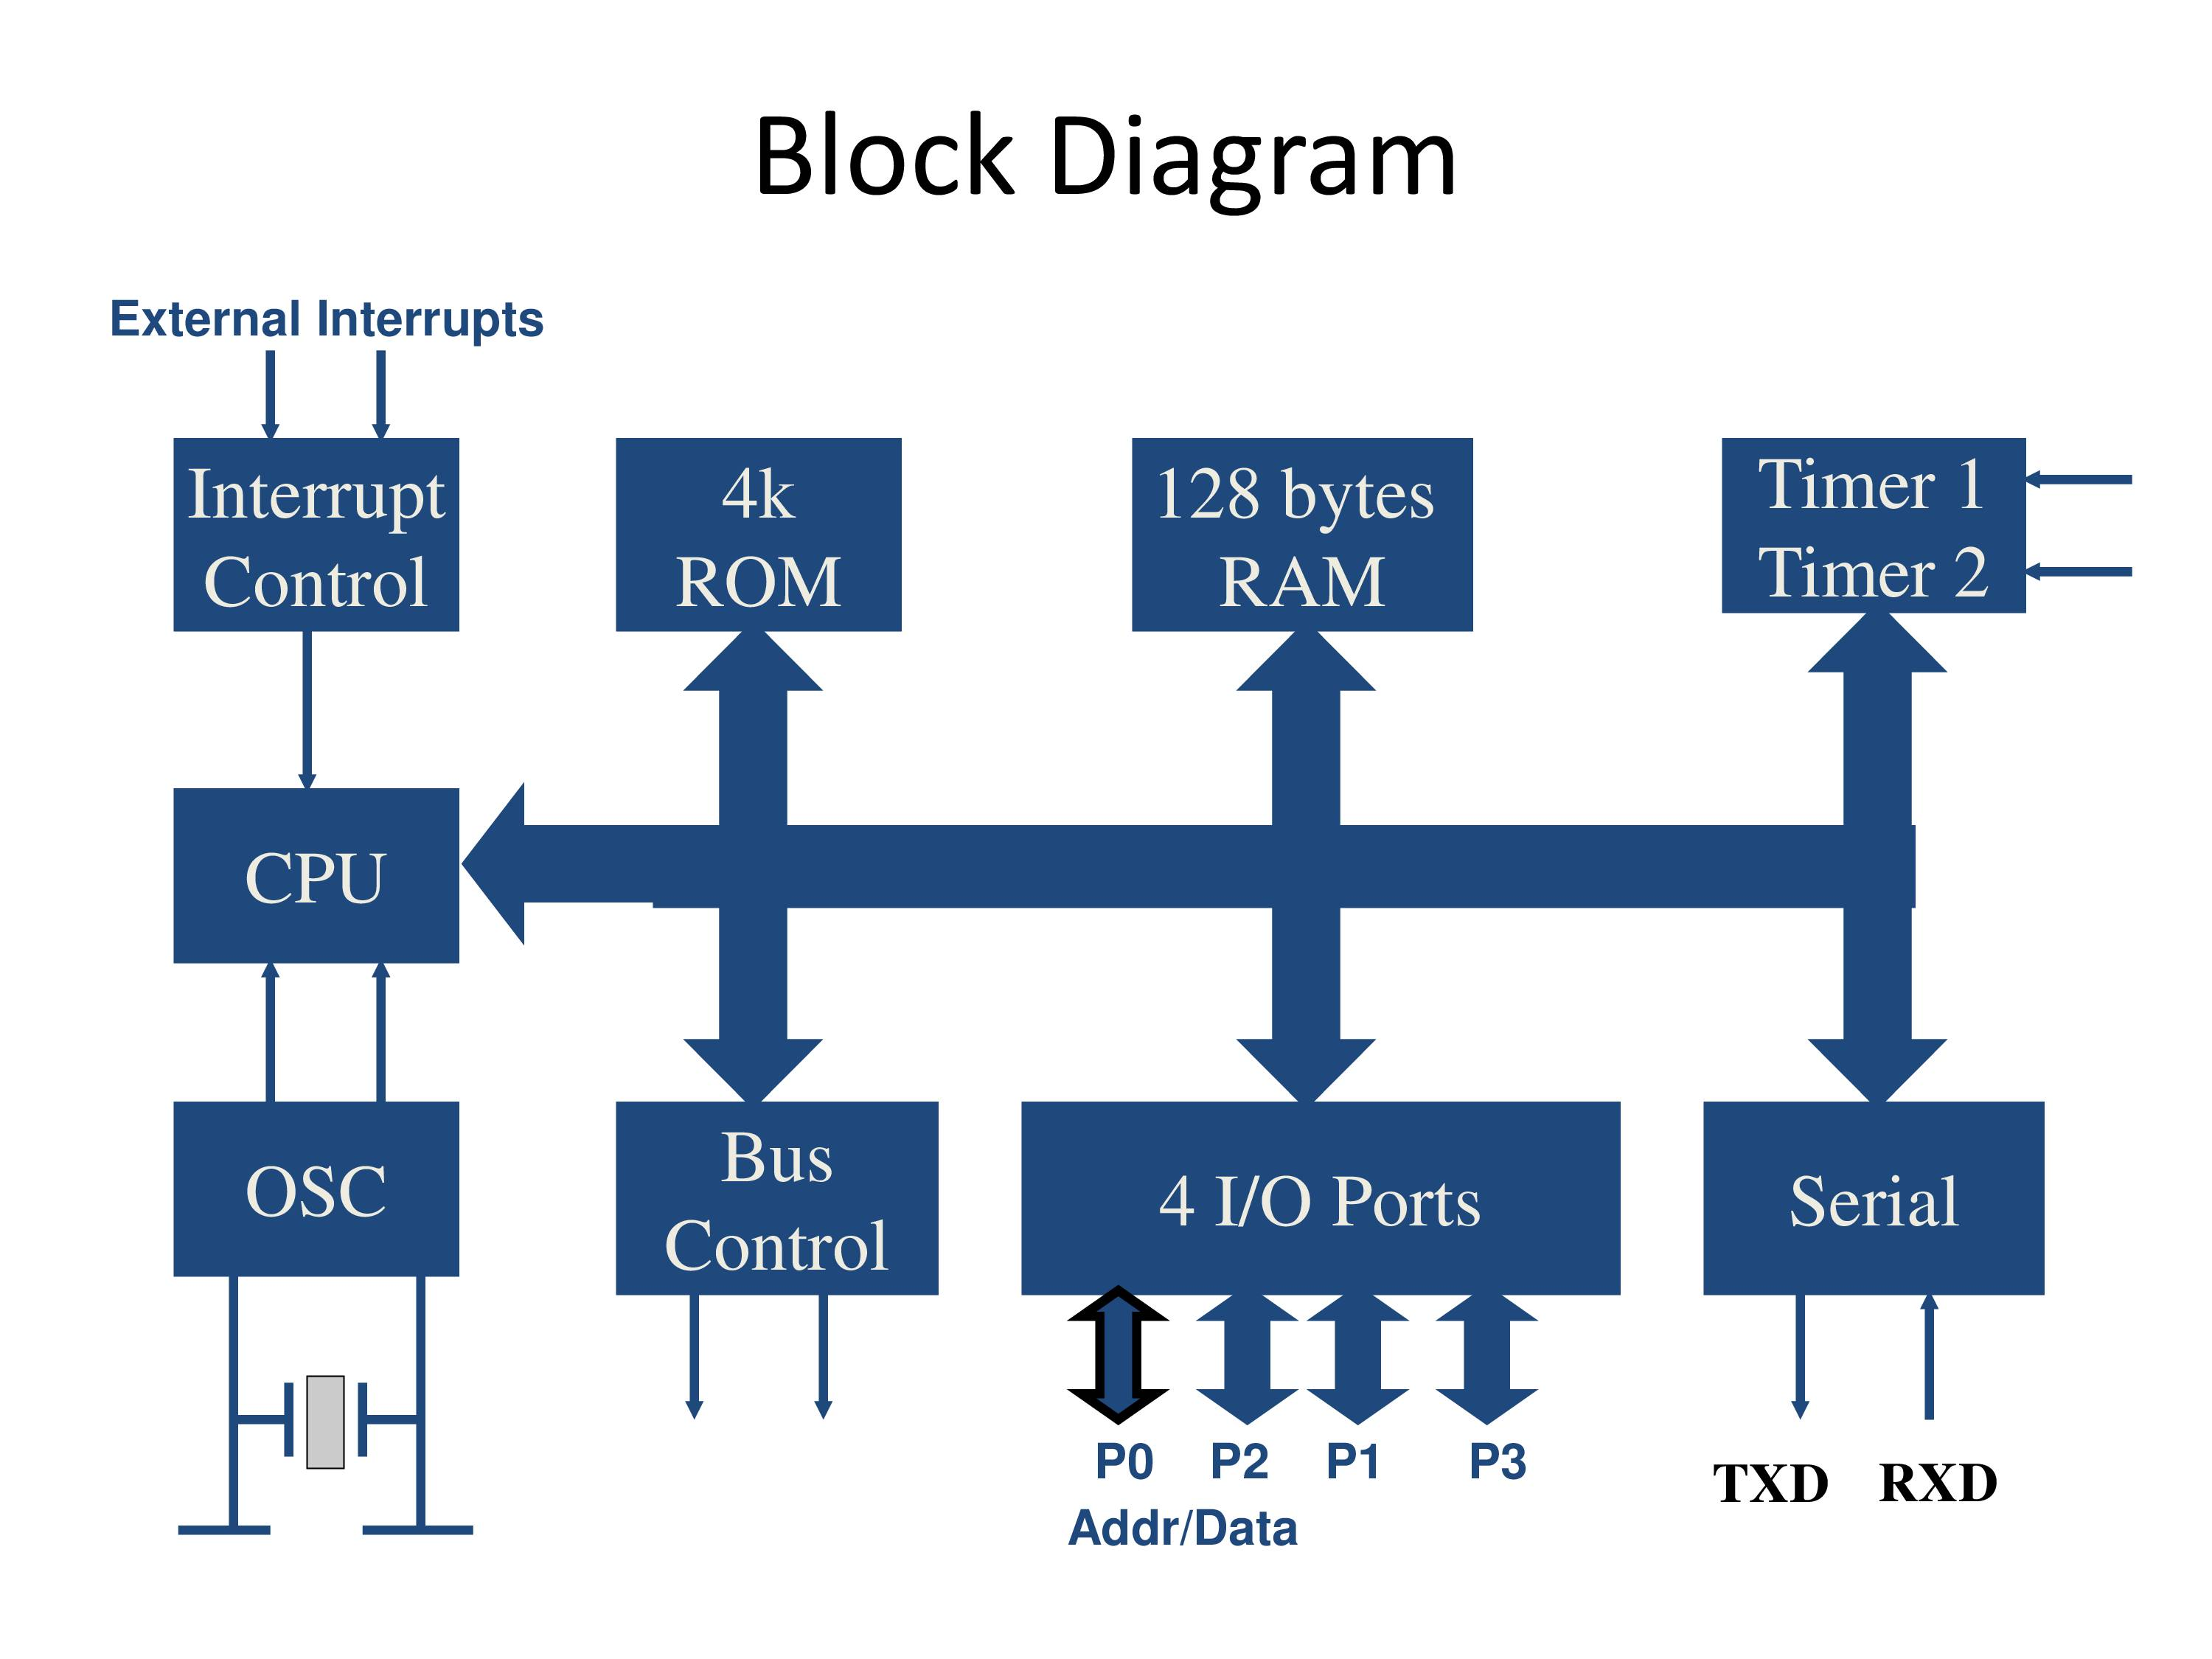
\includegraphics[scale=0.52,cframe=blue 0.5pt 3pt]{./block_diagram.jpg}
    \textit{\caption{Block diagram of 8051 microcontroller}}

\end{figure}

\subsection{7-Segment LED Display}
A seven segment display module is an electronic device used to display digital numbers and
it is made up of seven LED segments. LEDs are PN-junction diodes which emit energy by a process called electroluminescence.
Because of the small size of the LEDs, it is really easy for a number of them to be connected together to make a unit like seven segment display.
The light energy is emitted as ‘photons’ when it is forward biased by a voltage applied across its junctions.
In a seven segment display module, seven LED s are arranged in a rectangle. Sometimes,
an additional LED is seen in a seven segment display unit which is meant for displaying a decimal point.

Features of seven segment Display:-

\begin{itemize}
    \item Available in two modes Common Cathode (CC) and Common Anode (CA)
    \item Available in many different sizes like 9.14mm,14.20mm,20.40mm,38.10mm,57.0mm and 100mm (Commonly used/available size is 14.20mm)
    \item Available colours: White, Blue, Red, Yellow and Green (Res is commonly used)
    \item Low current operation
    \item Better, brighter and larger display than conventional LCD displays.
    \item Current consumption : 30mA / segment
    \item Peak current : 70mA
\end{itemize}

The displays common pin is generally used to identify which type of 7-segment display it is. As each LED has two connecting pins,
one called the “Anode” and the other called the “Cathode”, there are therefore two types of LED 7-segment display called: Common Cathode (CC) and Common Anode (CA).
The difference between the two displays, as their name suggests,
is that the common cathode has all the cathodes of the 7-segments connected directly together and the common anode has all the anodes of the 7-segments connected together
\begin{figure}[H]
    \centering
    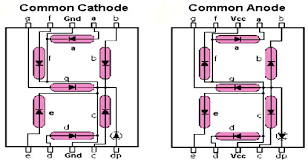
\includegraphics[scale=1.1,cframe=blue 0.5pt 3pt]{./Common cathode vs common anode.png}
    \textit{\caption{Common cathode vs Common anode 7 segment display}}
\end{figure}


\begin{figure}[H]
    \centering
    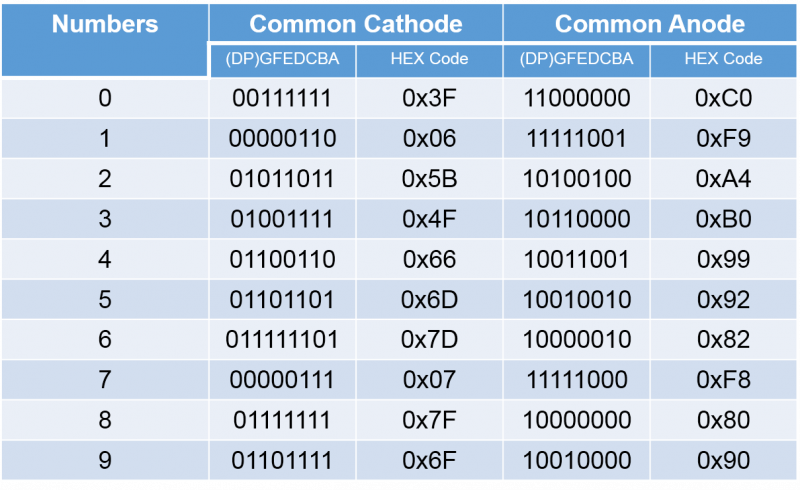
\includegraphics[scale=0.65,cframe=blue 0.5pt 3pt]{./Dispaly codes.png}
    \textit{\caption{Lookup table for Common anode and Common Cathode}}
\end{figure}

\subsection{Applications of Seven Segment Display}
\begin{itemize}
    \item Used in applications where font size is required to be bigger
    \item Microcontroller Independent, hence used in small circuit projects
    \item Used in combination with four segments to display measurement/sensor value  with four characters
    \item Has bright illumination, hence used where display are required to work in low light or dark conditions
\end{itemize}

\subsection{Timers in 8051}
The basic 8051 has two on-chip timers that can be used for
timing duration or for counting external events. Interval timing
allows the programmer to perform operations at specific
instants in time. Since the microcontroller operates at a specific
frequency, we could work out exactly how much iterations of
the time delay was needed to give us the required delay. Their application could be in communication for  generating  rectangle  pulses,  watchdog  timer,  in  manufacturing industry  for  counting objects,  measuring  intervals,  etc.  There  are  two  different  types  of timer:  Interval  timer  and Counter.
5
\begin{figure}[H]
    \centering
    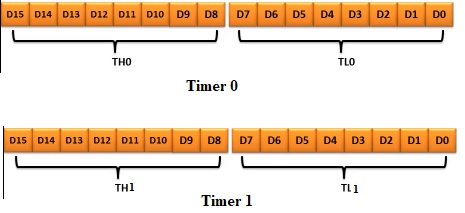
\includegraphics[scale=0.79,cframe=blue 0.5pt 3pt]{./t0t1.jpg}
    \caption{T0, T1 Timer Register}
\end{figure}

Two timers, namely Timer 0 and Timer 1 are 16 bits timer
and since 8051 has an 8-bit architecture, each 16-bits timer is
accessed as two separate registers of low byte and high byte.
The low byte register is called TL0/TL1 and the high byte
register is called TH0/TH1.

\subsection{Timer Mode Register(TMOD)}
TMOD is a 8-bit register whose lower 4 bits are for Timer 0 and upper
4 bits are for Timer 1.
It  is  byte  addressable  only,  which  is loaded  at  the  very beginning  of  a  program  to  initialize  a  timer's  mode.
In each case, the lower 2 bits are used to
set the timer mode and upper 2 bits to specify the operation.
\begin{itemize}
    \item \textbf{Timer Mode 0}
          Mode  0is identical  for  Timer  0  and  Timer  1.  Both  timers  work  as  13-bit counters;an  interrupt is generated  when  counter  overflows.  It  takes  8192  input  pulses  to  generate  the  next interrupt. Timers  use  8-bits  of  THi  and  5  lower  bits  of  TLi.  After  timer  overflows  TFi(Timer flag  in TCON) is set, hence an interrupt occurs.

    \item \textbf{Timer Mode 1}
          This mode is similar to mode 0. This timer uses all 8 bits of THi and 8 bits of TLi. So it is a 16-bit counter which can take 65536 input pulses to generate the next interrupt.

    \item \textbf{Timer Mode 2}
          In  this  mode,  the  timers  are  8  bits  auto  reload  type.  The  timer  is  operated by  TLi, when TLi overflows again it is automatically loaded by THi. So the initial value is loaded to the THi register at first.

    \item \textbf{Timer Mode 3}
          In this mode, only timer 0 can be used. This is also called split timer mode. Timer 0 operates  TL0  and  TH0  as  two  separate  8  bit  timers/counters.  Timer  0with  TL0  is  operated with TF0 and TR0 while timer 0 with TH0 is operated with TF1and TR1.

\end{itemize}

\begin{figure}[H]
    \centering
    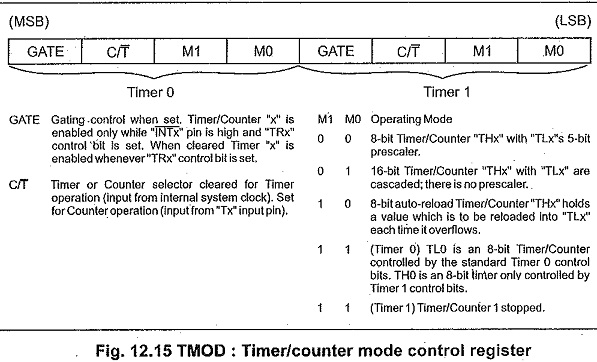
\includegraphics[scale=0.89,cframe=blue 0.5pt 3pt]{./Timer mode.jpg}
    \caption{Timer mode control register}
\end{figure}

\subsection{Timer Control Register (TCON)}
The 8051 microcontroller has one 8-bit register that holds the timer flags, interrupt ags and timer run control bit. This register is bit addressable and is used by both timers as well as interrupts. The timers use the upper4-bits while interrupts use the lower 4-bits.


\begin{figure}[H]
    \centering
    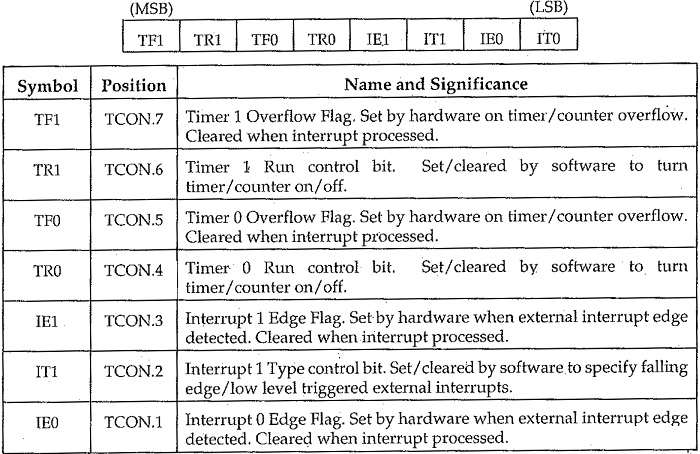
\includegraphics[scale=0.89,cframe=blue 0.5pt 3pt]{TCON.jpg}
    \caption{Timer Control Register (TCON)}
\end{figure}

\subsection{Clock Sources for Timer}
\textbf Using  TMOD  register,  timer operation  is  selected,  and timer  is clocked from an oscillator. Frequency for timer is $1/12^{th}$ the frequency of the crystal attached to the 8051 microcontroller, which is equivalent to 921.6 KHz (frequency of an oscillator is 11.0592  MHz).  This  is  so  as  in8051  microcontroller,  12  oscillator  periods constitute  a machine cycle. Hence machine cycle period is 1.085 microseconds.

\section{Objectives}
To enable us to write assembly language code for the 8051/8052 micro-controller capableof:
\begin{itemize}
    \item Applying timers in different timing modes.
    \item Implementing accurate delays using timers.
\end{itemize}


\section{Equipment Required}

\begin{itemize}
    \item Hardware:  8051 or 8052 micro-controller development board, Jumper cables

    \item Simulation  Software:  KEIL,  Vision-Embedded  development  tool, Proteus  Design Suite –Professional PCB layout, circuit design and simulation tool

    \item In-System Programming (ISP) Software: ProgISP –An in-system-programmable tool to load HEX  files in to micro-controller

    \item Device Drivers: LibUSB –Application controlling data transfer to/from USB devices
\end{itemize}


\pagebreak

\section{LAB problems}
%%%%%%%%%%%%%%%%%1111111111111111
\begin{Q}
    {
        Generate a periodic square wave having a period of 15 ms and a duty cycle of 20 \% . The waveform should be produced at pin zero of port two (P2.0). The XTAL frequency is 11.0592 MHz. Observe the waveform on an oscilloscope and measure the ON and OFF timers.
    }
\end{Q}

\begin{figure}[H]
    \centering
    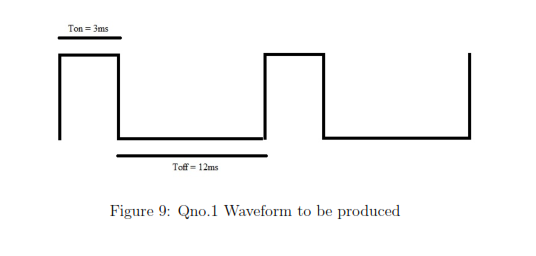
\includegraphics[scale=0.89,cframe=blue 0.5pt 3pt]{1 output.png}
    \caption{Waveform to be generated for Problem 1}
\end{figure}

\begin{figure}[H]
    \centering
    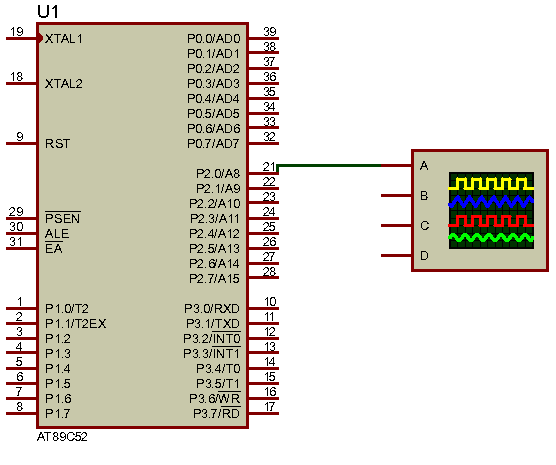
\includegraphics[scale=1.7,cframe=blue 0.5pt 3pt]{1.PDF}
    \caption{Proteus Schematic Problem no.1}
\end{figure}

\begin{enumerate}
    \item \textbf {Using Timer 1 in mode 0 (13-bit timer mode)}
          \anscode{1.a}{1a.a}{1a.c}


    \item \textbf {Using Timer 0 is mode 1 (16-bit timer mode)}

          \anscode{1.b}{1b.a}{1b.c}

    \item \textbf {Using Timer 1 in mode 2 (8-bit auto-reload timer mode)}

          \anscode{1.c}{1c.a}{1c.c}

    \item \textbf {Using Timer 0 (TL0) in mode 3 (8-bit split timer mode)}
          \anscode{1.d}{1d.a}{1d.c}

\end{enumerate}



\textbf{OUTPUT:}
All Outputs are Screenshot of Proteus Simulation.
Observation for mode 0, mode 1, mode 2 and  mode 3 are below . Due to some error perfect measurement cannot be taken . we have to generate a periodic square wave
having a period of 15 ms and duty cycle of 20 \%. So, total on
time of square wave per period $T_{ON}$ is 3ms while $T_{OFF}$ is 12 ms
we have made a delay of 3 ms and used it for both on and off cycle. For off cycle, delay is looped four times as off time is four times of on time.

\begin{figure}[H]
    \centering
    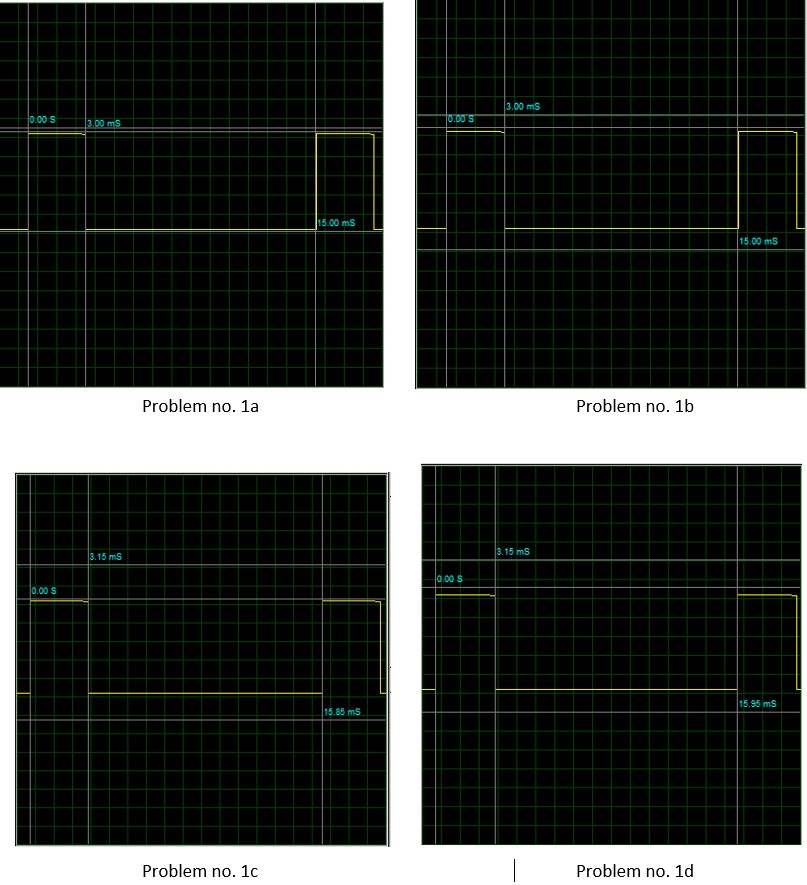
\includegraphics[scale=1,cframe=blue 0.5pt 3pt]{Prob1 graph.jpg}
    \caption{Graphs Problem no.1}
\end{figure}


\pagebreak
%%%%%%%%%%%%%%%%%%%%%22222222222222222222222222

\begin{Q}
    {
        Generate the periodic waveform as shown in figure 11. The waveform should be produced at pin zero of port zero (P0.0). The XTAL frequency is 11.0592 MHz. Observe the waveform on an oscilloscope and measure the ON and OFF times.
    }
\end{Q}

\begin{figure}[H]
    \centering
    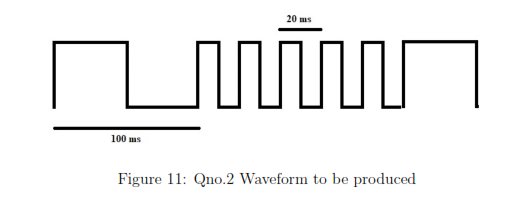
\includegraphics[scale=1,cframe=blue 0.5pt 3pt]{2output.png}
    \caption{Waveform to be generated for Problem 2}
\end{figure}


\begin{figure}[H]
    \centering
    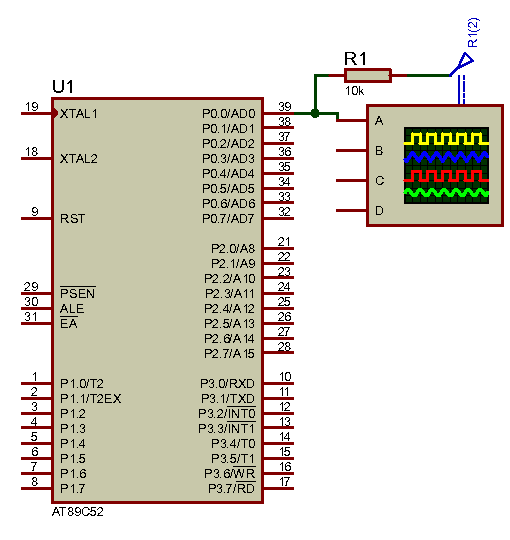
\includegraphics[scale=1.6,cframe=blue 0.5pt 3pt]{2.PDF}
    \caption{Proteus Schematic Problem no.2}
\end{figure}


\begin{enumerate}
    \item \textbf {Using Timer 0 and mode 0 (13-bit timer mode) }
          \anscode{2.a}{2a.a}{2a.c}


    \item \textbf {Using Timer 1 in mode 1 (16-bit timer mode) }

          \anscode{2.b}{2b.a}{2b.c}

    \item \textbf {Using Timer 0 in mode 2 (8-bit auto-reload timer mode) }

          \anscode{2.c}{2c.a}{2c.c}

    \item \textbf {Using Timer 0 (TH0) in mode 3 (8-bit split timer mode) }
          \anscode{2.d}{2d.a}{2d.c}

\end{enumerate}



\textbf{OUTPUT:}
There are two waveforms that we have top produce. First waveform has on and off cycle of 50 ms while second waveform has on and off cycle of 10 ms. In above program, two separate delays are made for 50 ms and 10 ms delay by providing different values in timer register.Observation for mode 0, mode 1, mode 2 and  mode 3 are below . Due to some error perfect measurement cannot be taken .
\begin{figure}[H]
    \centering
    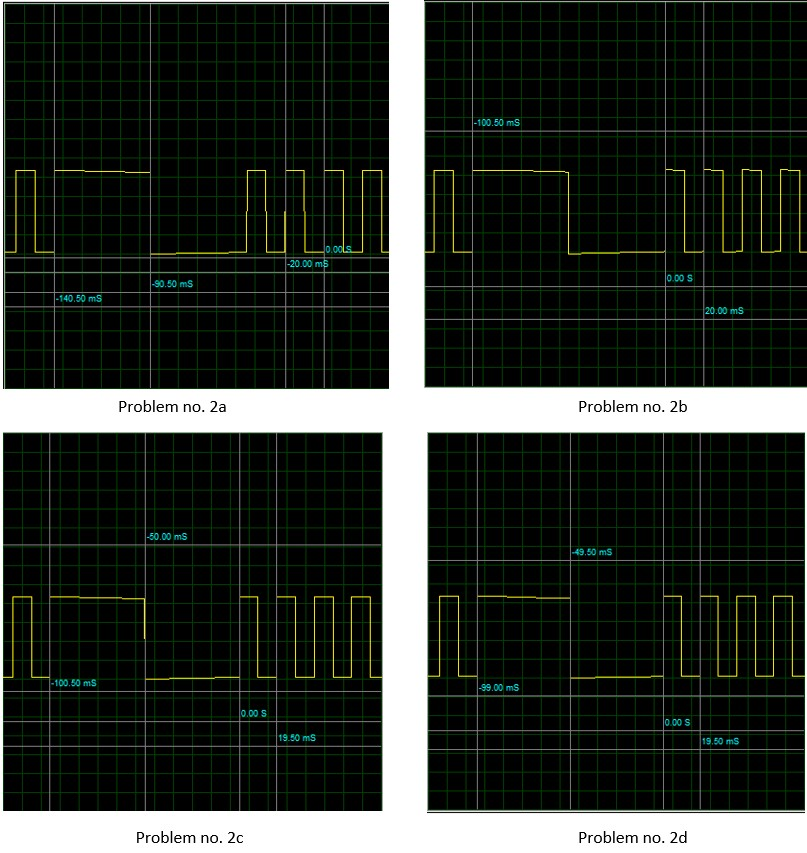
\includegraphics[scale=1,cframe=blue 0.5pt 3pt]{prob2 graph.jpg}
    \caption{Graphs Problem no.2}
\end{figure}


%%%%%%%%%%%%%%%%%%%%%


\pagebreak

%%%%%%%%%%%%%%%%%33333333333333333333333333333333
\begin{Q}
    {
        Design a digital minutes and seconds in double digit format. The clock should count from 00:00 to 59:59 and repeat. Time should be displayed in decimal format using four 7-segment LED units. A decimal point should separate minutes from seconds. Use an appropriate timer and timer mode. Use port 0 (P0) to send data to 7-segment LED units. Use transistors as switches to activate or deactivate the 7-segment LED units using pins 0, 1, 2 and 3 of port 2 (P2.0, P2.1, P2.2, P2.3).
    }
\end{Q}


\begin{figure}[H]
    \centering
    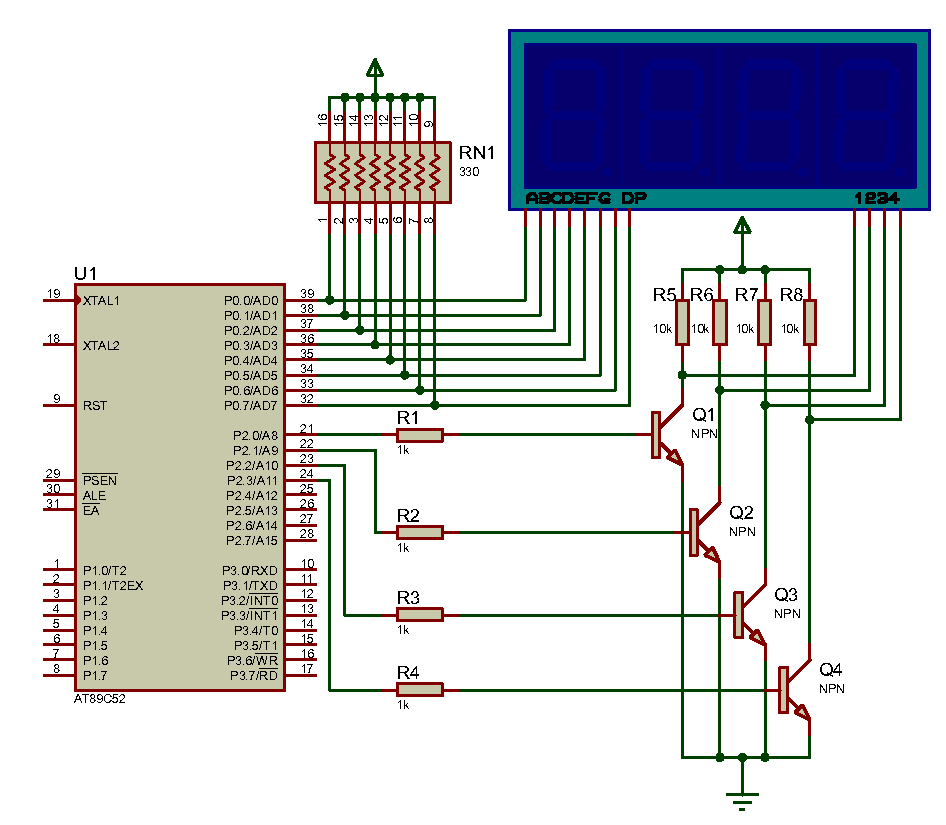
\includegraphics[scale=0.94,cframe=blue 0.5pt 3pt]{3.PDF}
    \caption{Proteus Schematic Problem no.3}
\end{figure}


\anscode{3}{3.a}{3.c}



\textbf{OUTPUT:}
Outputs include some snaps taken during that 60 minute period. here delay is used to make clock more accurate. the delay has ti=o be minimum to avoid flickering of LED.programming is done in binary format and we need to convert binary values to decimal equivalent while displaying the digits in LED unit.it also consist of hexadecimal to decimal converter sub-routine, display sub-routine, LED pattern selection sub-routine for efficient programming. ther is decimal point in between minute and second.
\begin{figure}[H]
    \centering
    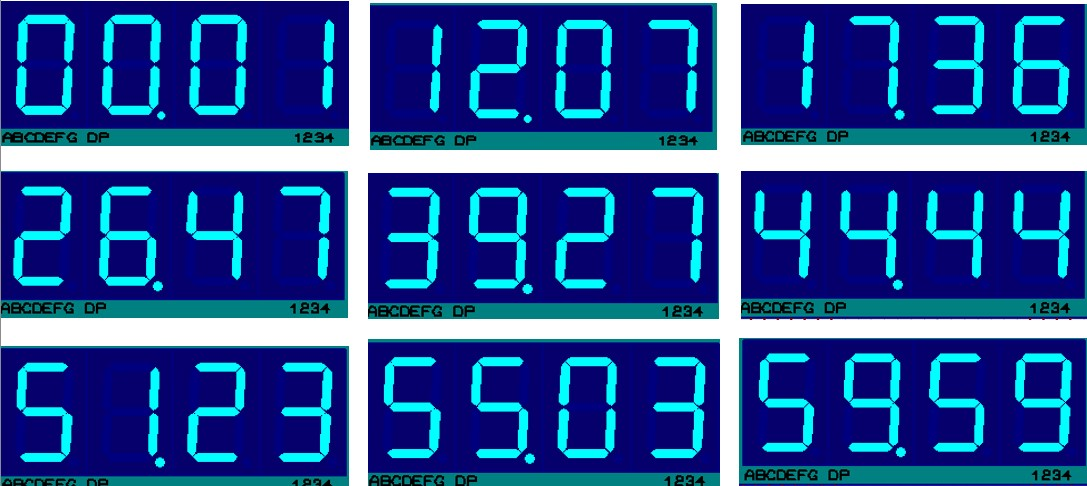
\includegraphics[scale=0.75,cframe=blue 0.5pt 3pt]{prob3 time.jpg}
    \caption{Timer Outputs}
\end{figure}

%%%%%%%%%%%%%%%%%%%%%

\section{Conclusion}

In this Lab we program timers of 8051/8052 in Microcontroller in C and Assembly Language. we performed various waveform using delay in Timers available in 8051/8052 microcontroller. Kiel IDE is used to generate HEX file from both Assembly and C language and Proteus to simulate the whole circuit.All codes ,schematic and Outputs are included in the report.








\end{document}